\newenvironment{dlblock}{\par\medskip\noindent\begin{minipage}{\linewidth}}{\end{minipage}\par\smallskip}
\subsubsection{从调阈值到让模型学习}
前一章我们自己规定了“什么算红色”“多大的轮廓留下来”。不过，数字写得歪一点、光照换一下，规则就不那么好写了。这时候可以换一种办法：给程序看一些图片，同时告诉它正确答案，让它调整内部参数，学出从图片到答案的映射。这就是本章要动手做的监督学习（supervised learning）。我们先识别手写数字，把训练、保存、重新使用走完，再去碰赛场数据；否则环境和数据一齐出问题，你很难知道该先修谁。

神经网络（neural network）可以用于回归预测、图像分类、目标检测和语言等任务，不能按“一维预测、二维识别”划分用途。这里识别的是整张小图属于哪个数字，叫分类（classification）；找出大图里物体的位置还要输出框，叫检测（detection）。模型本质上仍是一个带参数的函数，训练让它在数据上表现更好，并不自动保证新图片也能识别好。

先用一个不用神经网络的小实验看这件事。本卷 \path{examples/dl/lenet-training-demo} 是完整工程，下面全部源码都在相应位置展示，README 给出最短命令。先看 \texttt{fit\_demo}：五个训练点带小扰动，四个独立验证点来自 $y=x^2$，分别拟合一、二、四阶多项式。均方误差（mean squared error，MSE）为 $\frac1n\sum_i(\hat y_i-y_i)^2$。
\begin{example}[训练点记住了，下一张呢]
在项目目录运行 \texttt{python fit\_demo.py}，比较两列误差。四阶能穿过全部训练点，但本例验证误差比二阶大；只盯着训练成绩就会选错。程序里的点是教学数据，图不是神经网络的训练曲线。
\end{example}
\begin{dlblock}
\lstinputlisting[numbers=left,language=Python,caption={fit\_demo.py}]{examples/dl/lenet-training-demo/fit_demo.py}
\end{dlblock}
\begin{figure}[H]
\centering
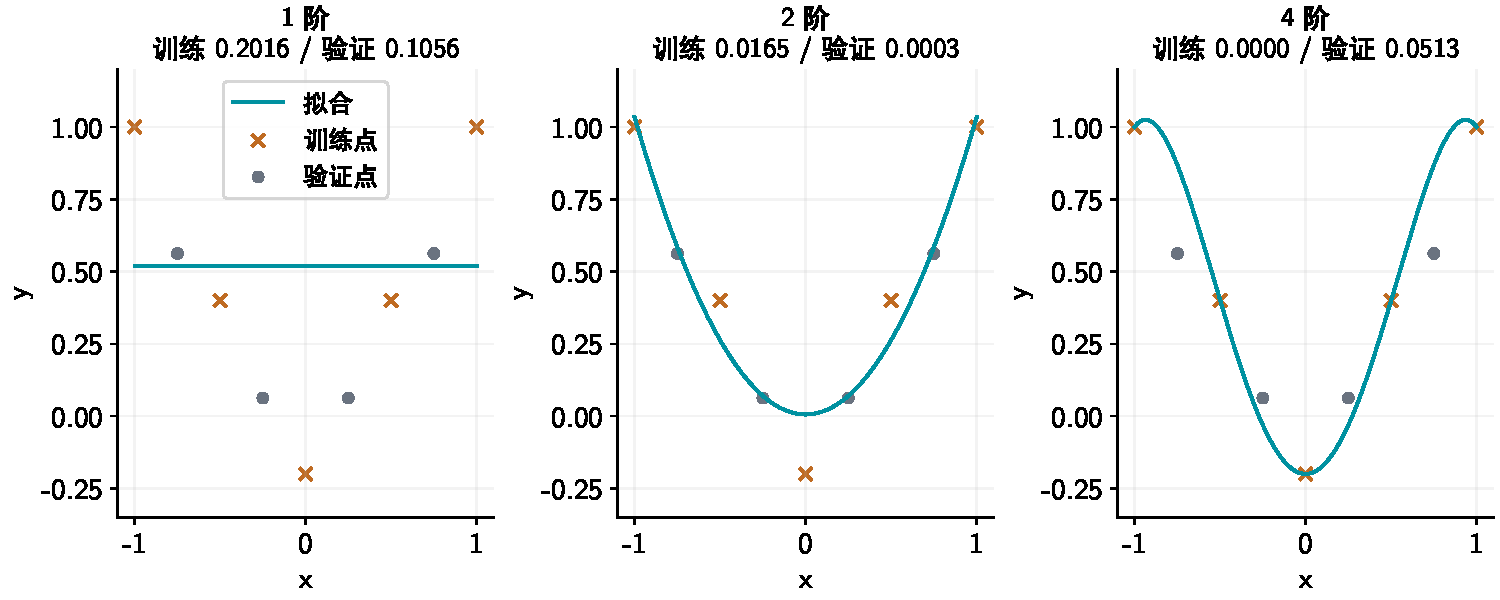
\includegraphics[width=0.98\textwidth]{images/dl_fit_revised.pdf}
\caption{同一组训练点和独立验证点的多项式实验，标出实际 MSE}
\label{fig:v2-dl-fit}
\end{figure}
欠拟合（underfitting）意味着模型连训练数据的规律都没有学好；过拟合（overfitting）则是训练表现很好，新的数据表现却差。图 \ref{fig:v2-dl-fit} 中先看训练点，再看灰色验证点。遇到后者，我们可以检查数据是否有代表性，尝试增强、正则化或早停；“把训练图片删少一些”不是通用解法。
\begin{exercise}\label{ex:v2-dl-fit}
将训练点扰动全部改成零，重新比较三个阶数的训练和验证 MSE。说明四阶模型是否一定过拟合，以及为何不能只凭模型复杂就下结论。
\end{exercise}
\begin{conclusion}
训练集用于更新参数，验证集用于选择配置与停止时机，测试集留到最后评价。训练误差小不等于泛化好，验证误差也不能证明所有赛场场景都可靠；把同一段视频的相邻帧分到训练和验证两边，很容易得到看起来漂亮的成绩。
\end{conclusion}

\subsubsection{先把 Python 环境选对}
卷一已经讲过虚拟环境。你可以继续用 Conda，也可以按下面的 venv 方法新建一个；不需要为了学习网络再配一遍整个系统。在 Distrobox 里先进入 Ubuntu，再进入工程目录。安装通用形式是 \texttt{python -m pip install [选项] 包名}；\texttt{-m pip} 使用当前解释器的包管理器，\texttt{==版本} 固定组合，\texttt{--index-url} 选择构建索引。
\begin{example}[先在 CPU 上把闭环跑通]
从项目目录执行。固定 PyTorch 2.6.0 与 torchvision 0.21.0，作为本章已验证的复现组合，不表示它们是最新版本。最后应看到解释器路径、两个版本与 \texttt{torch.Size([2,3])}。
\begin{tbash}
sudo apt install python3-venv
python3 -m venv .venv
source .venv/bin/activate
python -m pip install torch==2.6.0 torchvision==0.21.0 --index-url https://download.pytorch.org/whl/cpu
python -c "import sys,torch,torchvision; print(sys.executable,torch.__version__,torchvision.__version__,torch.ones(2,3).shape)"
\end{tbash}
\end{example}
如果终端能运行而 IDE 找不到 torch，先检查 IDE 选择的解释器是不是这个 \texttt{.venv/bin/python}。不是每个 import 错误都值得重装显卡驱动。CPU 包的 \texttt{torch.cuda.is\_available()} 为 False 很正常，需要 CUDA 时另选构建。
\begin{exercise}\label{ex:v2-dl-env}
分别在已激活与未激活虚拟环境的终端运行版本检查，记录解释器路径或实际导入错误。说明编辑器与终端版本不一致时先改哪项设置。
\end{exercise}

\subsubsection{数据：图片、标签和批量怎样配合}
MNIST 提供 60000 张训练来源图片和 10000 张测试图片，都是 $28\times28$ 手写数字灰度图，标签为 0 到 9。我们从前者固定划出 55000 张训练、5000 张验证，不拿测试集决定训练轮数。首次需要网络下载，torchvision 会校验资源；下载失败时先处理连接或缓存，不要用随机标签假装训练成功。

Dataset 保存取样规则，DataLoader 按批量（batch）交付图片与标签。ToTensor 对这里的 PIL 灰度图把 0--255 转成浮点 0--1，并增加通道维；Normalize 再按 $(x-\mathrm{mean})/\mathrm{std}$ 处理。本例沿用 MNIST 参考常数 0.1307、0.3081，没有从测试集重新估计。部署仍须使用相同处理，不是把图片 resize 成 28 就结束了。
\begin{example}[把三个集合分开]
data.py 返回三个 loader，训练打乱、评估不打乱，固定随机生成器让划分可重现。\texttt{train\_limit}=128 只缩小训练子集，验证和测试不动。后面的 train 入口直接调用它，显示首批形状。
\end{example}
\begin{dlblock}
\lstinputlisting[numbers=left,language=Python,basicstyle=\footnotesize\ttfamily,caption={data.py}]{examples/dl/lenet-training-demo/data.py}
\end{dlblock}
\begin{exercise}\label{ex:v2-dl-data}
以 \texttt{--train-limit 128 --batch-size 50 --epochs 1 --out smoke50} 运行入口。预测三个训练批量大小，核对训练样本数；解释最后一批为什么不能按 50 个样本计算平均损失。
\end{exercise}

\subsubsection{卷积、池化与激活：先算一个小窗口}
搭网络之前，我们先看看层到底做什么。卷积层（convolution layer）用可训练的核提取局部特征。同一个核在不同位置复用参数，各输出通道使用自己的核；多输入通道还要把各通道结果求和并加偏置。Conv2d 实际使用不翻转核的互相关（cross-correlation）约定，工程里仍习惯叫卷积。图 \ref{fig:v2-dl-conv} 的左上输出为 19，你可以拿四个乘法核对，不必先背一页公式。
\begin{equation}
Y_{o,i,j}=b_o+\sum_c\sum_{a=0}^{k_h-1}\sum_{b=0}^{k_w-1}
 W_{o,c,a,b}X_{c,is_h+a-p_h,js_w+b-p_w}.
\end{equation}
越界位置按零填充处理。膨胀率为 1 时，高度输出为
$\left\lfloor(n_h+2p_h-k_h)/s_h\right\rfloor+1$，宽度同理；$p_h$ 是每侧填充量，$s_h$ 是步幅（stride）。核不必是奇数，图中 $2\times2$ 就能算，只是 $3\times3$、$5\times5$ 很常见。
\begin{figure}[H]
\centering
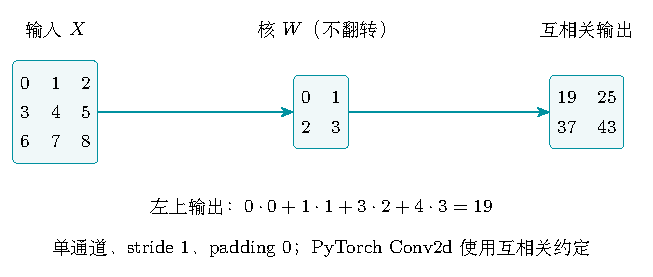
\includegraphics[width=0.9\textwidth]{images/dl_conv_revised.pdf}
\caption{不翻转核的互相关，保留原图的输入、核与输出数值}
\label{fig:v2-dl-conv}
\end{figure}
池化层（pooling layer）也滑动窗口，不过没有这里的可训练核权重：最大池化取最大值，平均池化取平均值。它常用于减少空间尺寸，对局部位置变化有一定容忍，但不保证任意平移后结果都相同。图 \ref{fig:v2-dl-pool} 两个结果分别来自原输入，窗口是 $2\times2$、步幅是 1；本章网络中步幅为 2，别照抄图的尺寸。
\begin{figure}[H]
\centering
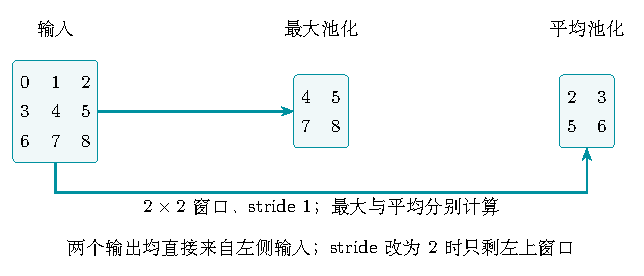
\includegraphics[width=0.9\textwidth]{images/dl_pool_revised.pdf}
\caption{同一输入的最大和平均池化，右侧不是再处理中间结果}
\label{fig:v2-dl-pool}
\end{figure}
激活函数（activation function）引入非线性。只叠多个线性层而不加非线性，最终仍能合并为一个仿射变换。我们用 ReLU（rectified linear unit，修正线性单元）：$\mathrm{ReLU}(x)=\max(0,x)$，负输入输出零，不是删除参数。另一个常见函数 $\mathrm{sigmoid}(x)=1/(1+e^{-x})$ 把有限实数压到 0--1 之间；本章多类别输出没有使用它。
\begin{example}[公式算完，让程序再算一次]
运行 \texttt{python ops\_demo.py}，互相关为 19/25/37/43，最大池化为 4/5/7/8，平均为 2/3/5/6；随后比较两种激活对负数、零、正数的结果。
\end{example}
\begin{dlblock}
\lstinputlisting[numbers=left,language=Python,caption={ops\_demo.py}]{examples/dl/lenet-training-demo/ops_demo.py}
\end{dlblock}
\begin{exercise}\label{ex:v2-dl-ops}
把两个池化调用的步幅改为 2，预测尺寸和数值后运行；再将核改为全 1，核对互相关。两次修改分别保存，不要把窗口、步幅和核一起改得认不出来。
\end{exercise}

\subsubsection{搭建 LeNet：每一层都能对上形状}
现在我们把这些层串起来。nn.Module 管理参数与子模块，\texttt{\_\_init\_\_} 创建层，forward 定义数据经过它们的顺序。本例是 LeNet 风格的教学网络，两组卷积/ReLU/最大池化后接三个全连接层（fully connected layer）；没有照搬原始 LeNet-5 的激活、汇聚和输出形式。旧图常见的是 32 输入，本章 MNIST 为 28 输入，图 \ref{fig:v2-dl-lenet} 将两条尺寸链分开了。

Conv2d(1,6,5) 的位置参数是输入通道、输出通道和核大小；MaxPool2d(2) 默认步幅等于核大小。尺寸为 $28\to24\to12\to8\to4$，一个样本最终有 $16\times4\times4=256$ 个特征。flatten(1) 保留第零维批量，展平其余维；Linear(84,10) 给十类输出未归一化分数（logits），暂时没有概率。
\begin{figure}[H]
\centering
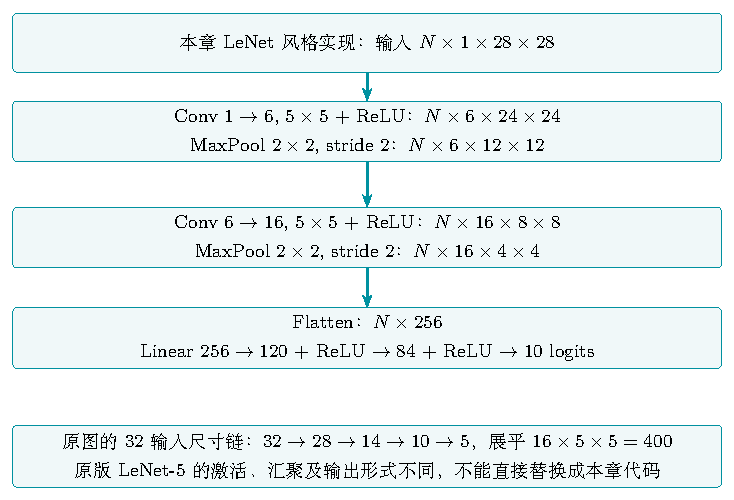
\includegraphics[width=0.92\textwidth]{images/dl_lenet_revised.pdf}
\caption{本章形状与原图 32 输入的区别，$N$ 为批量大小}
\label{fig:v2-dl-lenet}
\end{figure}
\begin{example}[先前向，再训练]
运行 \texttt{python model.py}，看到特征 \texttt{(2,16,4,4)}、展平 \texttt{(2,256)}、分数 \texttt{(2,10)}。Sequential 将连续层组合为容器，作用与同序逐个调用一致；特征与分类器分开，方便你检查中间形状。
\end{example}
\begin{dlblock}
\lstinputlisting[numbers=left,language=Python,basicstyle=\footnotesize\ttfamily,caption={model.py}]{examples/dl/lenet-training-demo/model.py}
\end{dlblock}
\begin{exercise}\label{ex:v2-dl-shape}
将入口输入改为 $32\times32$，记录特征与展平形状，再看分类器报错。手算并修改第一层 Linear 输入数，使它输出 \texttt{(2,10)}；此变体不要覆盖后面的 28 输入模型。
\end{exercise}

\subsubsection{损失、反向传播和优化器各做什么}
前向能输出分数，不过随机参数还不会认数字。损失函数（loss function）衡量预测与标签的差距，反向传播（backpropagation）按链式法则计算参数梯度，优化器（optimizer）才用梯度更新参数。这三步不要混成“调用 backward 就学会了”。

本章交叉熵（cross entropy）针对单个正确类别 $y$：
$L=-\log\bigl(e^{z_y}/\sum_j e^{z_j}\bigr)$，$z$ 是 logits。CrossEntropyLoss 内部完成稳定的 log-softmax，给它整数标签与原分数；你若先 softmax，就让它把概率又当分数处理，损失含义变了。
\begin{example}[分数、概率和损失别重复加工]
运行 \texttt{python loss\_demo.py}，交叉熵与负对数正确类概率一致，约 0.16985；提前 softmax 后约 0.65785。随后打印的是分数梯度，不是更新后的分数。
\end{example}
\begin{dlblock}
\lstinputlisting[numbers=left,language=Python,caption={loss\_demo.py}]{examples/dl/lenet-training-demo/loss_demo.py}
\end{dlblock}
简单梯度下降为 $\theta\leftarrow\theta-\eta\nabla_\theta L$，学习率（learning rate）$\eta$ 控制步长。我们先用一个参数算清楚，再在网络中使用 Adam。Adam 用梯度的一、二阶矩估计调整更新量，不保证必然稳定或达到全局最优；学习率、批量与轮数仍按验证结果选择。
\begin{example}[梯度算出来了，参数还没动]
\texttt{grad\_demo} 的 $w=0$、$L=(2w-4)^2$，第一次梯度 -16；重新建图反传但不清梯度，变为 -32。清零后以学习率 0.1 更新一步，$w=1.6$、损失约 0.64。运行 \texttt{python grad\_demo.py} 核对三次状态。
\end{example}
\begin{dlblock}
\lstinputlisting[numbers=left,language=Python,caption={grad\_demo.py}]{examples/dl/lenet-training-demo/grad_demo.py}
\end{dlblock}
\begin{exercise}\label{ex:v2-dl-grad}
把 SGD 学习率改为 0.05，手算清零后一步的参数和损失，再运行。说明保留 -32 梯度会有什么不同，以及 backward 与 step 的分工。
\end{exercise}

\subsubsection{训练与评估：不用训练时的状态考自己}
每批先清梯度，前向求分数和损失，再反传、更新；评估只前向统计。engine 将两者放在同一函数，是否传入 optimizer 决定行为。损失按样本数累加，因为最后一批可能较小，直接平均每批均值会给小批量同样的权重。

train/eval 改变 Dropout、BatchNorm 等层行为，\texttt{no\_grad} 关闭梯度记录，两者不是同一开关。本例 LeNet 没有这两类层，数值可能看不出区别，但仍保留正确评估路径，否则以后换网络就容易踩坑。
\begin{example}[两个开关分开看]
运行 \texttt{python mode\_demo.py}。训练状态即使在 \texttt{no\_grad} 中，Dropout 仍将部分输入置零并缩放；eval 输出全 1，但输入需要梯度时仍保留梯度关系。代码在 Dropout 后 clone 一次，避免 p=0 直接返回原输入时把原输入的 \texttt{requires\_grad} 误当作新计算图。eval 与 \texttt{no\_grad} 一起使用才是此处推理状态。
\end{example}
\begin{dlblock}
\lstinputlisting[numbers=left,language=Python,caption={mode\_demo.py}]{examples/dl/lenet-training-demo/mode_demo.py}
\end{dlblock}
\begin{example}[一套循环负责训练和验证]
下面的 engine 被 train 实际调用。评估不会清梯度、反传或更新，也不记录计算图；统计返回样本数，能与集合大小对照。完整运行紧接在入口后。
\end{example}
\begin{dlblock}
\lstinputlisting[numbers=left,language=Python,basicstyle=\footnotesize\ttfamily,caption={engine.py}]{examples/dl/lenet-training-demo/engine.py}
\end{dlblock}
\begin{exercise}\label{ex:v2-dl-mode}
将 Dropout 概率改为 0，重复三种状态。输出相同是否说明两个开关可以互相代替？指出 engine 控制层状态和梯度记录的两条语句。
\end{exercise}
\begin{conclusion}
forward 给预测，loss 衡量差距，backward 算梯度，step 更新参数，\texttt{zero\_grad} 防止意外累加。train/eval 控制层行为，梯度记录另有开关。训练保留反向所需中间值，较大批量或网络可能占用更多内存/显存；显存不足时先缩小批量并检查是否留住了旧计算图，不能只看参数文件大小。
\end{conclusion}

\subsubsection{完整入口：小批量检查，再恢复训练}
文件职责已经清楚了：data 给集合，model 给结构，engine 执行一轮，train 配置、选模型与保存，infer 在另一进程使用结果。其他 demo 只为了缩小观察难点，不参与主线训练。项目目录如下：
\begin{tbash}
lenet-training-demo/
  model.py  data.py  engine.py  train.py  infer.py
  fit_demo.py  ops_demo.py  loss_demo.py  grad_demo.py  mode_demo.py
  device_demo.py  nms_demo.py  export_compare.py  benchmark.py
  requirements-export.txt  README.md
\end{tbash}
入口前半段的 --data 是缓存目录，--out 是结果目录，默认 CPU、一个线程、批量 64、三轮；train-limit 0 是完整训练子集。先移动模型，再创建优化器，每批输入与标签也移到同一设备。固定种子便于本机对照，不保证跨设备和版本逐位相同。
\begin{dlblock}
\lstinputlisting[numbers=left,language=Python,firstline=1,lastline=40,basicstyle=\footnotesize\ttfamily,caption={train.py：参数与准备}]{examples/dl/lenet-training-demo/train.py}
\end{dlblock}
后半段逐轮记录训练与验证，只在验证损失改善时保存。结束后载入选中的参数，最后评价一次测试集；测试没有回头影响选择。除了权重，还保存结构名称、归一化与类别表，避免留下不知道怎样使用的“存档”。metrics.json 记录版本、配置与曲线。
\begin{dlblock}
\lstinputlisting[numbers=left,language=Python,firstline=41,firstnumber=41,basicstyle=\footnotesize\ttfamily,caption={train.py：选模型、保存与最终评价}]{examples/dl/lenet-training-demo/train.py}
\end{dlblock}
\begin{example}[先确认代码能绕回来]
从工程目录执行。128 张一轮的首批为 \texttt{(64,1,28,28)}、标签 \texttt{(64,)}、输出 \texttt{(64,10)}；随后恢复完整训练。每轮 train 记录为 55000 样本，valid 为 5000，最终 test 为 10000。
\begin{tbash}
python train.py --epochs 1 --train-limit 128 --out smoke
python train.py --epochs 3 --out runs
python infer.py --index 0 1 2
\end{tbash}
\end{example}
\begin{note}
再次用同一输出目录会覆盖 best.pth 与 metrics.json，比较实验请换 --out。128 张只检查流程，准确率低不说明环境坏了，也别凭这点样本给模型下结论。训练启动后无需一直按运行按钮，等一轮统计出来再判断。
\end{note}
\begin{figure}[H]
\centering
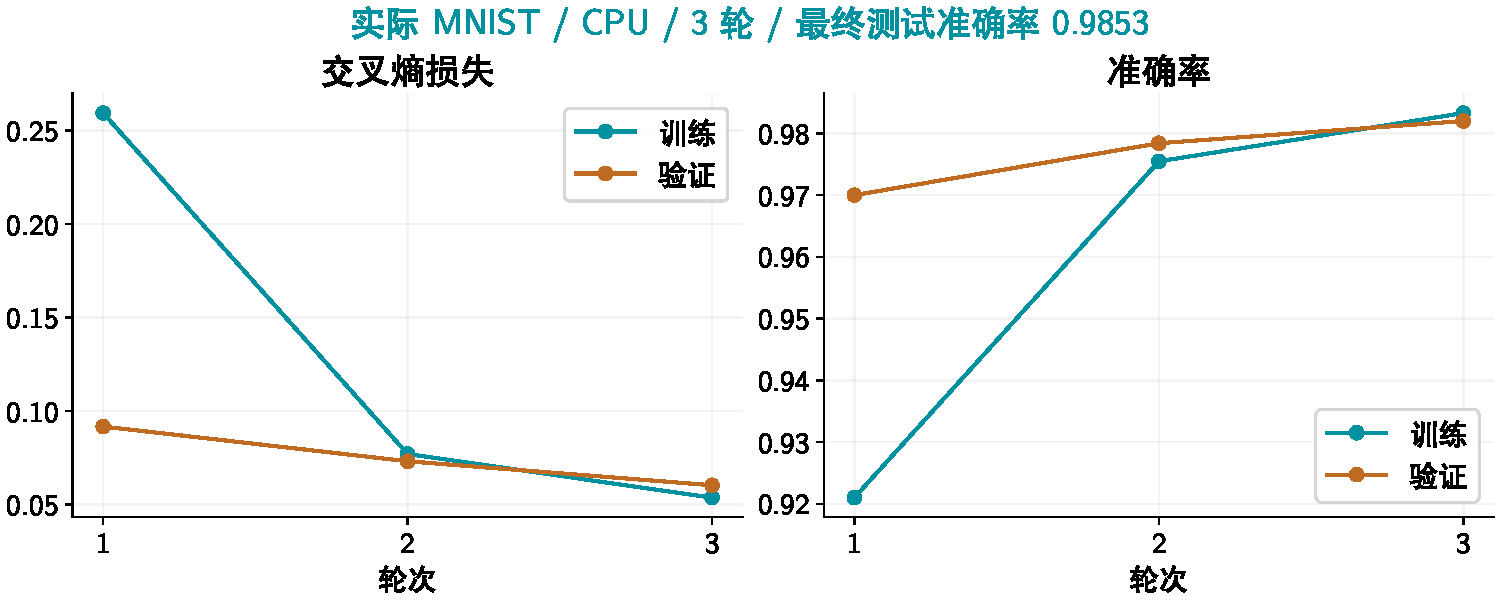
\includegraphics[width=0.96\textwidth]{images/dl_curve_revised.pdf}
\caption{本次 CPU 三轮完整训练的真实记录，成绩随版本与配置变化}
\label{fig:v2-dl-curve}
\end{figure}
图 \ref{fig:v2-dl-curve} 来自 Ubuntu 24.04/PyTorch 2.6.0 CPU 实际运行，最终测试准确率 0.9853。它说明此教学任务的结果，不证明装甲板数字也能直接识别；真实数据的裁剪、类别、模糊和光照不同，赛场训练见卷三。
\begin{exercise}\label{ex:v2-dl-train}
完成小规模与完整训练，记录版本、集合样本数及每轮验证损失。根据 metrics 判断保存哪一轮，解释只看最后一轮训练损失为什么不能替代这个选择。
\end{exercise}

\subsubsection{保存与加载：参数还需要使用说明}
参数文件有了，不过 \texttt{state\_dict} 主要是参数与持久缓冲，不替你保存完整网络定义、预处理和类别含义。加载时先创建相同结构，再填参数；仅把后缀从 .pth 改成 .onnx 可不会施展格式转换魔法。

infer 使用保存的结构标记与归一化，对指定测试样本输出十个分数和预测类别，取最大分数索引。想显示概率时再 softmax，概率大小也不自动等于校准后的可靠程度。\texttt{map\_location}='cpu' 让 CUDA 权重能在 CPU 读取，\texttt{weights\_only}=True 限制加载形式；仍应使用自己训练或可信来源的文件。
\begin{example}[换一个进程读存档]
运行 \texttt{python infer.py --index 0 1 2}，三行给索引、真标签、预测与分数。检查者可指定 0--9999 索引。--checkpoint 换权重路径，--data 与训练缓存一致，不需要再训练。
\end{example}
\begin{dlblock}
\lstinputlisting[numbers=left,language=Python,firstline=1,lastline=16,basicstyle=\footnotesize\ttfamily,caption={infer.py：结构与参数}]{examples/dl/lenet-training-demo/infer.py}
\end{dlblock}
\begin{dlblock}
\lstinputlisting[numbers=left,language=Python,firstline=17,firstnumber=17,basicstyle=\footnotesize\ttfamily,caption={infer.py：指定样本与分数}]{examples/dl/lenet-training-demo/infer.py}
\end{dlblock}
\begin{exercise}\label{ex:v2-dl-load}
复制 model，将第一层 Linear 输入改为 400，再在变体工程用原权重运行 infer，记录报错。恢复结构后核对同一图片输出，说明改变归一化为什么可能不报错却改变预测。
\end{exercise}

\subsubsection{选用 CUDA：先确认构建和设备，再谈速度}
如果有可用 NVIDIA 显卡，可选 PyTorch CUDA 构建，让相同循环使用 GPU。CPU 包不会因装了驱动就变成 CUDA 包；PyTorch 附带的运行库也不是下一章的完整 nvcc 工具链。先查驱动，再从 \href{https://docs.pytorch.org/get-started/previous-versions/}{官方固定版本组合}选匹配构建，建议保留能用的 CPU 环境。
\begin{example}[本机可用时走相同训练路径]
在新环境安装下面已验证的组合，再进入相同工程。前提是驱动与容器能使用此 CUDA 构建。不能使用的机器继续 CPU 主线。
\begin{tbash}
python3 -m venv .venv-cuda
source .venv-cuda/bin/activate
python -m pip install torch==2.6.0 torchvision==0.21.0 --index-url https://download.pytorch.org/whl/cu126
python -c "import torch; print(torch.__version__,torch.version.cuda,torch.cuda.is_available())"
python train.py --epochs 1 --train-limit 128 --device cuda --out gpu-smoke
python device_demo.py
\end{tbash}
\end{example}
\texttt{device\_demo} 用主线 runs/best.pth 的相同参数与输入比较 CPU/CUDA，不拿两个随机网络硬比。本次 Distrobox 的 RTX 3070 Ti Laptop GPU 实际跑通 CUDA 12.6 构建；其他设备仍按实际检查。没有传输、预热与同步的计时，不能证明 GPU 更快。
\begin{dlblock}
\lstinputlisting[numbers=left,language=Python,caption={device\_demo.py}]{examples/dl/lenet-training-demo/device_demo.py}
\end{dlblock}
\begin{exercise}\label{ex:v2-dl-device}
记录两个环境的版本与可用性；有设备时跑 gpu-smoke 和同参数比较，提交设备名与误差。无设备时指出 train 移动模型、输入、标签的位置，如实写未完成 GPU 实测。
\end{exercise}

\subsubsection{从分类到检测：框还要解码和去重}
数字分类只输出类别分数，机器人检测还要告诉我们物体在哪。YOLO（You Only Look Once）是一类检测方法和多个实现的名字，不是永远相同的架构。图 \ref{fig:v2-dl-yolo} 保留原图历史 YOLOv5s 的 Focus/CSP/SPP、多尺度融合与三个预测尺度，用 \href{https://github.com/ultralytics/yolov5/blob/v1.0/models/yolov5s.yaml}{v1.0 配置}定位；608 输入对应 76、38、19 网格，255 来自三组 anchor 和 80 类，不能直接套任意新版。
\begin{figure}[H]
\centering
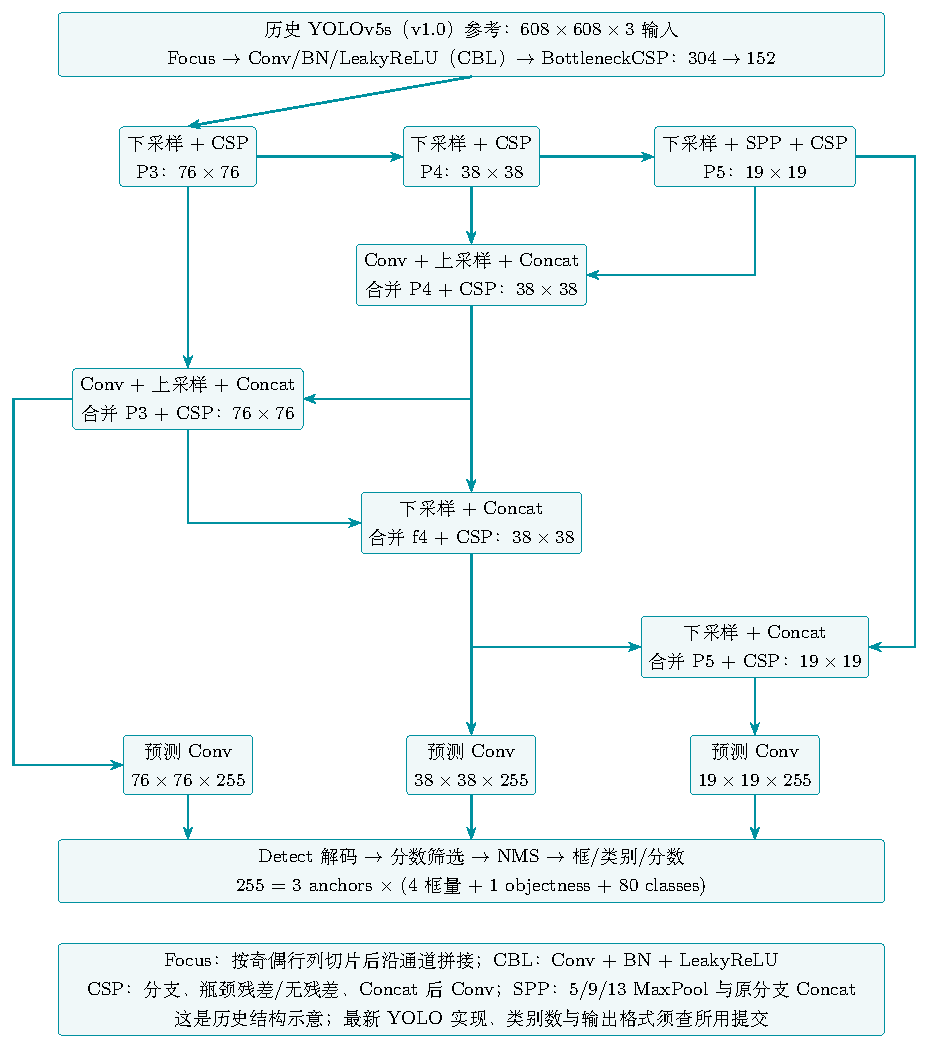
\includegraphics[width=0.88\textwidth]{images/dl_yolo_revised.pdf}
\caption{历史 YOLOv5s 的多尺度路径和模块含义，不是本章训练网络}
\label{fig:v2-dl-yolo}
\end{figure}
用现成框架仍须核对提交、许可、类别表、颜色与归一化、缩放/补边、输出解码。网络给候选框后，常用非极大值抑制（non-maximum suppression，NMS）去掉同类高重叠框；交并比（intersection over union，IoU）是交集面积除以并集面积。分数高不等于框正确，NMS 也不负责修错分类。
\begin{example}[三个同类框的去重]
运行 \texttt{python nms\_demo.py}，保留索引 0、2。前两个框 IoU 为 $81/119\approx0.681$，低分框被抑制；第三个在另一处。这是人工候选框后处理，没有训练好的 YOLO 权重，不要当检测成绩。
\end{example}
\begin{dlblock}
\lstinputlisting[numbers=left,language=Python,caption={nms\_demo.py}]{examples/dl/lenet-training-demo/nms_demo.py}
\end{dlblock}
\begin{exercise}\label{ex:v2-dl-nms}
将 IoU 阈值改为 0.8，预测保留索引后运行。说明改变的是去重条件还是网络预测；不同类别的重叠框能否直接沿用这个同类示例。
\end{exercise}

\subsubsection{部署入口：先核对数值，再测用时}
机器人程序可能使用不同语言、运行时和硬件。ONNX（Open Neural Network Exchange）用于交换计算图，OpenVINO、TensorRT 等可为目标设备转换或优化；算子支持、尺寸、精度与速度仍由实际模型和设备决定。.pth/.pt 常见于 PyTorch 保存，OpenVINO IR 常见 .xml/.bin，TensorRT 引擎常见 .engine，这些不能靠改名互换。

先做能核验的导出。依赖集中在 \path{requirements-export.txt}，固定 onnx 1.17.0 与 onnxruntime 1.20.1。随后 \texttt{export\_compare} 从主线权重读结构、预处理，用同一真实测试图分别在 PyTorch 与 CPU ONNX Runtime 前向，比较完整分数。输入固定 $1\times1\times28\times28$、opset 17；dynamo=False 明确此次实测路径，不靠新版默认值猜行为。
\begin{dlblock}
\lstinputlisting[numbers=left,caption={requirements-export.txt}]{examples/dl/lenet-training-demo/requirements-export.txt}
\end{dlblock}
\begin{example}[导出成功还要比较]
在 CPU 环境、项目目录执行。结果显示 \texttt{[1,10]}、最大绝对误差与类别，满足代码容差。默认写到已有 runs，换 --output 时确保父目录存在。
\begin{tbash}
python -m pip install -r requirements-export.txt
python export_compare.py
\end{tbash}
\end{example}
\begin{dlblock}
\lstinputlisting[numbers=left,language=Python,firstline=1,lastline=24,basicstyle=\footnotesize\ttfamily,caption={export\_compare.py：同一预处理输入}]{examples/dl/lenet-training-demo/export_compare.py}
\end{dlblock}
\begin{dlblock}
\lstinputlisting[numbers=left,language=Python,firstline=25,firstnumber=25,basicstyle=\footnotesize\ttfamily,caption={export\_compare.py：图与完整输出误差}]{examples/dl/lenet-training-demo/export_compare.py}
\end{dlblock}
onnx.checker 检查图，数值比较检查这些输入的实际输出，不能证明所有输入正确。当前图未包含外部预处理，部署须保存 mean/std、颜色、尺寸与类别表。查看结构可用 \href{https://netron.app/}{Netron}，导出限制查 \href{https://docs.pytorch.org/docs/2.6/onnx.html}{本章版本的导出文档}；结构能打开不是部署完成。

然后测 CPU 前向。计时器（benchmark）预热并多次测量，以中位数减少偶然波动；固定一个线程，比较批量 1 与 32。每样本成本与吞吐率说明批处理效率，单帧响应还包含预处理、排队、传输和后处理。CUDA 异步提交也不能直接用普通时钟相减测完整 GPU 用时，需要同步或事件计时。
\begin{example}[同一模型比较两个批量]
在有主线权重的 CPU 工程运行 \texttt{python benchmark.py}，报告每批毫秒、每样本毫秒、每秒样本数与线程数，不预先承诺快多少。
\end{example}
\begin{dlblock}
\lstinputlisting[numbers=left,language=Python,caption={benchmark.py}]{examples/dl/lenet-training-demo/benchmark.py}
\end{dlblock}
\begin{exercise}\label{ex:v2-dl-deploy}
换测试索引 1、2 分别导出比较，记录误差与类别。再把 benchmark 批量 32 改为 8，报告三个时间/吞吐指标，说明此计时没覆盖哪些单帧工作。
\end{exercise}
\begin{conclusion}
参数需要结构与预处理，交换图需要算子、尺寸与数值检查，部署还需要目标运行时、后处理与端到端计时。本章跑通 CPU ONNX Runtime 固定输入对照，OpenVINO/TensorRT 是后续目标，未实测就不写加速完成。
\end{conclusion}
到这里，我们能训练小网络、存下参数、在新进程识别指定样本，并跨运行时核对输出。神经网络在自瞄数字、装甲板与雷达感知中都有用，不过下一步应换成代表性真实数据与明确任务。想继续看自动求导与数据加载，可以顺着 \href{https://docs.pytorch.org/tutorials/beginner/basics/}{PyTorch 官方基础教程}查，先把当前闭环解释清楚再加新框架。
